\subsubsection{Data Access Layer}
Data Access Layer består af tre dele. Den første består af at modtage produktoversigter fra CentralServer. Den anden består af at sende information om gennemførte køb til CentralServer. Den tredje består af at denne salgskvitteringer efter køb er blevet gennemført

\begin{figure}[H]
	\centering
	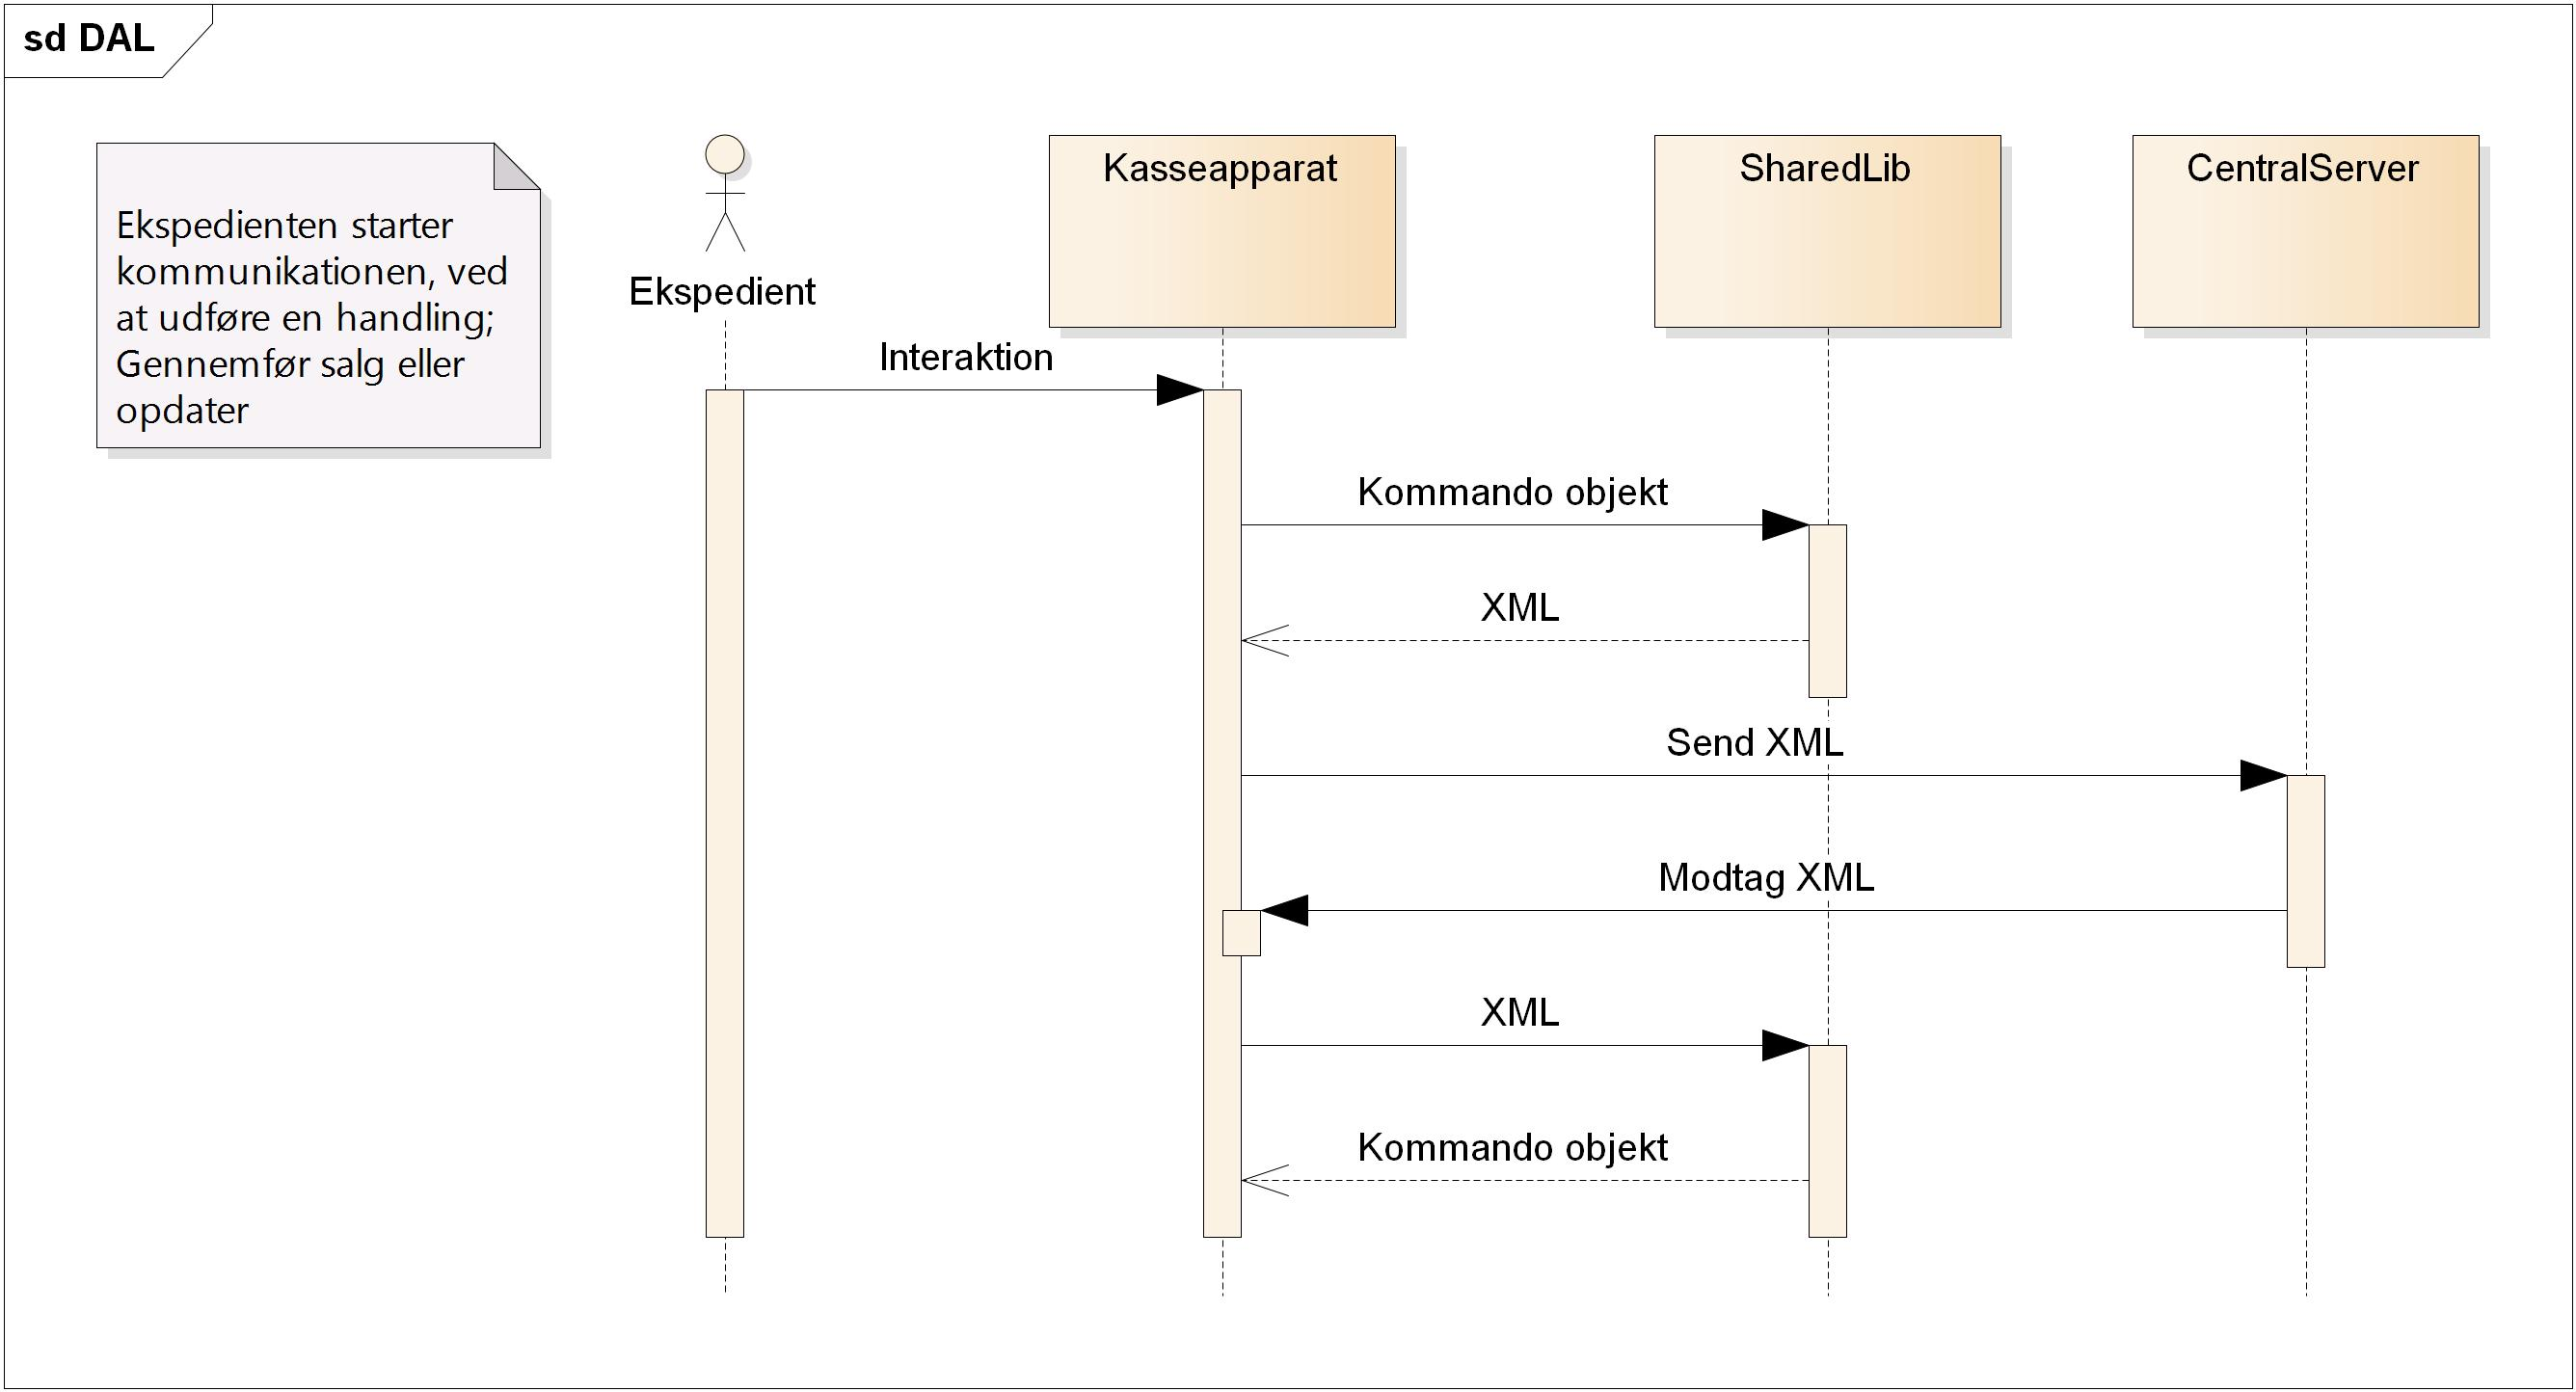
\includegraphics[width=\textwidth]{Projektbeskrivelse/DesignOgImplementering/Frontend/Pics/DALsq}
	\caption{Kommunikation til/fra CentralServer}
	\label{fig:KAtCS}
\end{figure}

Figur \ref{fig:KAtCS} viser et generelt eksempel på hvordan kommunikationen til CentralServer fungere. Ekspedienten gennemføre f.eks. et køb i brugergrænsefladen, herefter laves et kommando objekt, som encodes til en XML-streng ved hjælp af SharedLib. Denne XML streng sendes til CentralServer. Forventes et svar modtages dette i form af en XML string, denne decodes til kommando objekt, som inderholder informationen.\\
Oprettelse af salgskvitteringer foregår ved at der oprettes en tekst fil, navngivet efter tidspunkt for købet.


